\chapter{Contexte de travail}
\label{sec:context}

  Pour répondre à ces enjeux de passage à l'échelle et de consommation
  énergétique, l'équipe ALSOC du LIP6 participe à deux projets d'envergures:
  TSAR~\cite{tsar2008} et SHARP~\cite{sharp2012}. Le premier a pour but de
  fournir une architecture matérielle passant à l'échelle de plusieurs centaines
  de c\oe urs, tandis que l'autre se veut être capable de fournir un système
  d'exploitation pour gérer efficacement cette nouvelle architecture.

  Notre travail portera sur le multi-noyau ALMOS, et plus particulièrement sur
  la migration de tâches entre différentes instances du noyau. Nous allons dans
  un premier temps présenter l'architecture matérielle TSAR. L'étude de cette
  dernière est essentielle pour bien comprendre les enjeux d'ALMOS. Ensuite nous
  présenterons le noyau ALMOS, et notamment son cycle de vie, et enfin nous
  concluerons sur le travail que nous allons effectuer dans le cadre de ce
  stage.
  

  \section{L'architecture TSAR}
  \label{sec:tsar}

    TSAR est l'architecture d’un processeur multi-c\oe urs cc-NUMA homogène
    pouvant intégrer jusqu’à 1024 c\oe urs~\cite{greiner2009tsar}. Cette
    architecture est le résultat d’un projet de recherche européen
    MEDEA+~\cite{tsar2008} dont les principaux partenaires industriels sont
    BULL, Philips et THALES, et dont les partenaires académiques sont le LIP6 et
    le CEA-Leti. La figure \ref{fig:tsar} est un aperçu global de l'architecture
    TSAR. Il s'agit d'un ensemble de clusters interconnectés par un NoC
    (\textit{Network-On-Chip}) DSPIN (\textit{Distributed, Scalable,
      Predictable, Integrated Network}). Chaque c\oe ur dispose de ses propres
    caches L1 indexés en adresses physiques (données et instructions séparés) et
    d'une MMU (Memory Management Unit). La cohérence des caches de premier
    niveau de tous les c\oe urs ainsi que des TLB est assurée par un protocole
    matériel nommé DHCCP (\textit{Distributed Hybrid Cache Coherence
      Protocol}). Une description complète de cette architecture est disponible
    sur le site du projet TSAR~\cite{tsar2008web}.

    \begin{figure}[ht]
      \centering 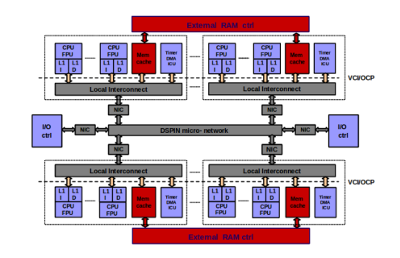
\includegraphics[scale=1]{include/img/tsar.png}
      \caption{Schéma global de l'architecture TSAR. Les clusters sont composés
        de quatre processeurs connectés entre eux sur un interonnect local,
        lui-même relié à différents périphériques (TTy, ICU, NIC,
        etc\ldots)~\citep{greiner2009tsar}.}
      \label{fig:tsar}
    \end{figure}

    Dans la suite de ce document, on considére la version TSAR-Leti comme étant
    l'architecture de base. Celle-ci contient 1024 processeurs réparti en 256
    clusters de 4 processeurs chacun. La mémoire vive est de 1To, et chaque
    cluster gère un segment de 4Go. Lors de la mise sous tension, c'est le
    cluster 0 qui est chargé d'initialiser tout le système.

  \section{Le noyau ALMOS}
  \label{sec:almos}

    Le noyau ALMOS~\cite{almaless2011almos} est un noyau monolithique
    expérimental developpé au LIP6 par l'équipe ALSOC depuis 2011. Sujet de
    thèse de Ghassan Almaless, le développement est maintenant à la charge de
    Mohamed Karaoui (système de fichiers) et Clément Devigne (exécution de
    machines virtuelles). Le but d'ALMOS est de répondre à la problématique
    évoquée de la localité des accès mémoires dans les machines cc-NUMA. Une des
    particularités dans les choix architecturaux d'ALMOS est d'avoir choisi de
    développer un noyau monolithique. Il respecte la norme
    POSIX~\cite{posix2013} et implémente différentes libraires:
    \texttt{libpthread, mpi, openMP}\ldots Le but premier d'ALMOS est de
    garantir un passage à l'échelle et une conservation de la localité des accès
    mémoires. Pour cela, le noyau intègre trois nouveaux mécanismes:
    \benumline \item les clusters managers \item les réplica-noyau \item une
    nouvelle stratégie d'allocation mémoire (\textit{Auto-Next-Touch})
    \eenumline.

    
    \subsection{Les cluster-manager}

      L'organisation distribuée du noyau ALMOS s’appuie sur les objets nommés
      \textit{cluster-manager}. L’objectif est d’une part, de décentraliser la
      gestion des ressources et d’autre part, d’assurer une localité d’accès
      mémoire lors de cette gestion. Un cluster-manager est un objet responsable
      de la gestion des ressources physiques (essentiellement c\oe urs et
      mémoire physique) d’un nœud cc-NUMA. Il existe autant de cluster-manager
      qu’il y a de clusters. Chacun d'eux est placé localement dans la mémoire
      physique de son n\oe ud. Comme l'illustre la
      figure~\ref{fig:cluster_manager}, ils contiennent, entre autre, un
      \textit{memory-manager} et un ou plusieurs \textit{core-manager}.  Le
      \textit{memory manager} est responsable de l'allocation et la gestion de
      la mémoire sur le cluster. Le \textit{core-manager} est responsable de la
      gestion d’un c\oe ur, et plus précisément de l'ordonnancement des tâches
      qui lui sont affectées. Il assure également la gestion des événements. %%Au
      %% sein de cet object, l'ordonnancement est assuré par un serveur
      %% d'ordonnancement appelé \textit{scheduler-server}, tandis que la
      %% gestion des événements est assurée par \textit{l'events-manager}.

      \begin{figure}[ht]
        \centering 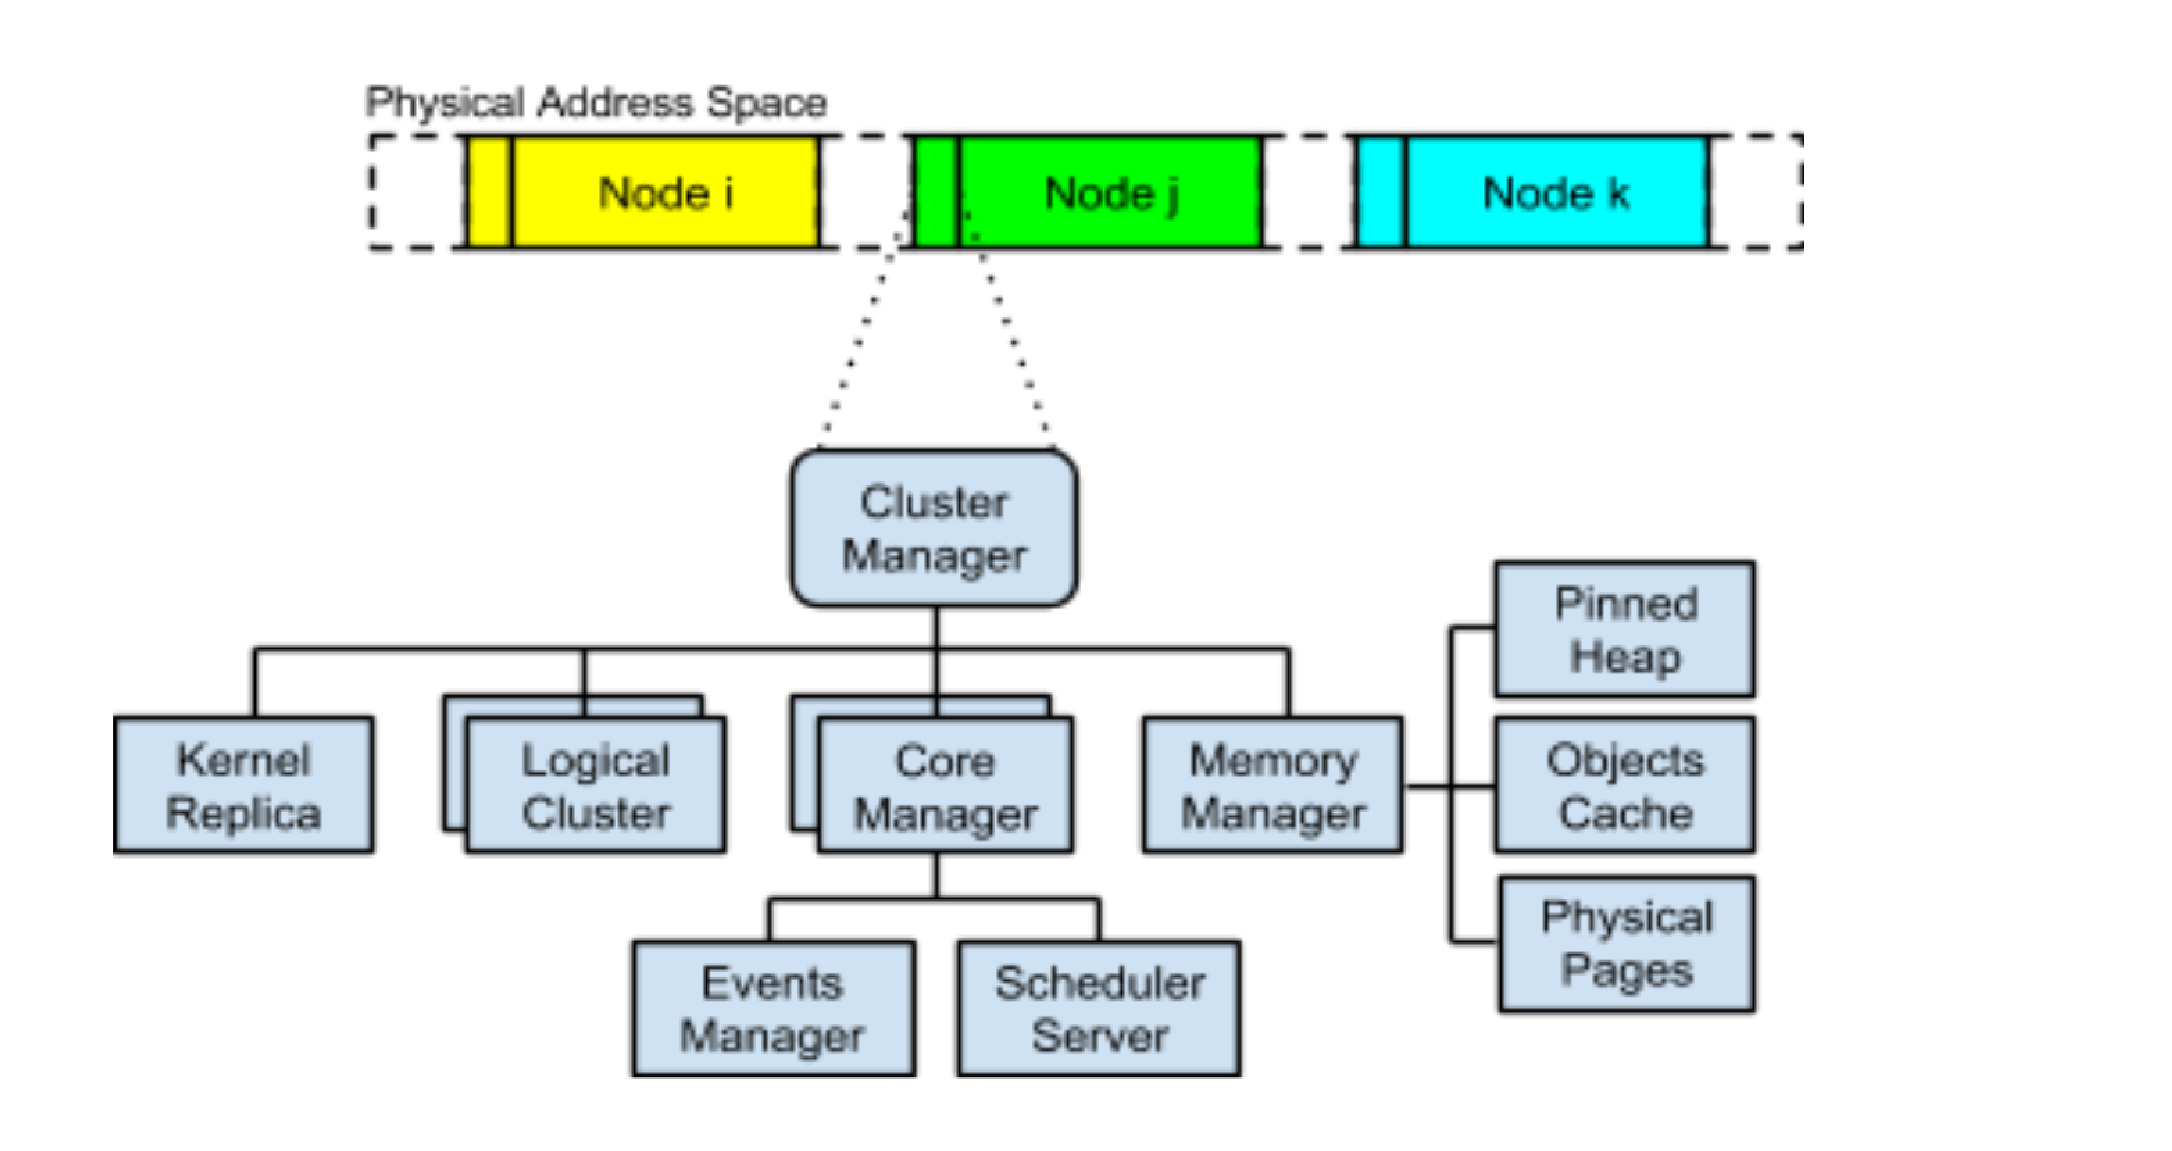
\includegraphics[scale=0.9]{include/img/cluster_manager}
        \caption{Un \textit{cluster manager} est un gestionnaire de ressources
          d'un n\oe ud cc-NUMA. Il est physiquement placé dans le banc mémoire
          du n\oe ud correspondant~\citep{almaless2014universite}.}
        \label{fig:cluster_manager}
      \end{figure}

      
    \subsection{Les réplicas noyau}

      Comme nous l'avons vu précédemment, l'architecture TSAR offre au système
      d'exploitation la notion de cluster.
      
      Dans l'espace d'adressage d'un processus, il y a un mapping sur certaines
      pages du noyau. Néanmoins, si le code et les données du noyau sont situés
      à un seul et unique endroit en mémoire physique, et que chaque processus
      mappe ces pages dans son espace virtuel, alors on paiera le coût de
      l'architecture NUMA à chaque appel système, puisque l'on devra accéder à
      des pages distantes.

      Afin de résoudre ce problème, la notion de réplica noyau a été introduite
      au sein des \textit{clusters-manager}. Un réplica noyau consiste à
      dupliquer le code du noyau et les données partagées dans les premières
      pages physiques de chaque cluster. Ces pages sont en lecture seule pour
      garantir la cohérence et la sécurité. Lors de la création d'un processus,
      les pages qui représentent le noyau correspondent aux pages physiques du
      cluster sur lequel le processus vient d'être créé.


  \section{Évolution du projet}

    \subsection{Limitations de la version initiale}
    
      Développé initialement pour une architecture 32 bits, le noyau ne peut pas
      supporter plus de 4Go de mémoire vive. L'objectif visé n'était pas de
      supporter le téra-octet de mémoire de TSAR, mais de supporter le passage à
      l'échelle de plusieurs centaines de c\oe urs. Ainsi, un des premiers
      problème d'ALMOS est le mapping de l'espace virtuel, qui se révèle être
      très simple. En effet, lors de la phase de boot, ce dernier va chercher à
      mapper le maximum de la mémoire physique du cluster de boot dans son
      espace virtuel. Contraitement aux noyaux ``classiques'', ALMOS s'accorde
      2Go d'espace virtuel au lieu de 1. Donc, si ce cluster possède (au moins)
      2Go de mémoire physique, l'ensemble du noyau est mappé dans ce seul
      cluster. Enfin, cela ne laisse que 2Go de mémoire virtuelle pour les
      applications utilisateur.

      
    \subsection{Contributions de François \citeauthor{guerret2014exploitation}}
      
      La gestion d'une telle quantité de mémoire fût le sujet de stage de
      François~\citet{guerret2014exploitation} en 2014. Ce dernier proposa
      différents changements pour ALMOS : \benumline \item réduire l'espace
      virtuel du noyau à 1Go \item répartir cet espace virtuel entre les
      clusters \item sortir de l'espace virtuel les structures de données du
      noyau de taille importante \eenumline. Ces changements sont représentés
      par la figure~\ref{fig:almos-guerret}.

      \begin{paragraph}{Répartition de l'espace d'adressage noyau:}
        Elle est calculée en fonction du nombre de clusters de l'architecture
        ($\frac{\text{Taille virtuelle}}{\text{Nb clusters}}$). Pour une
        architecture TSAR-Leti 40 bits, on dispose de 256 clusters, on a donc
        $\frac{1000}{256}\approx4$Mo d'espace virtuel pour le noyau par cluster.
      \end{paragraph}

      \begin{figure}[ht]
        \centering 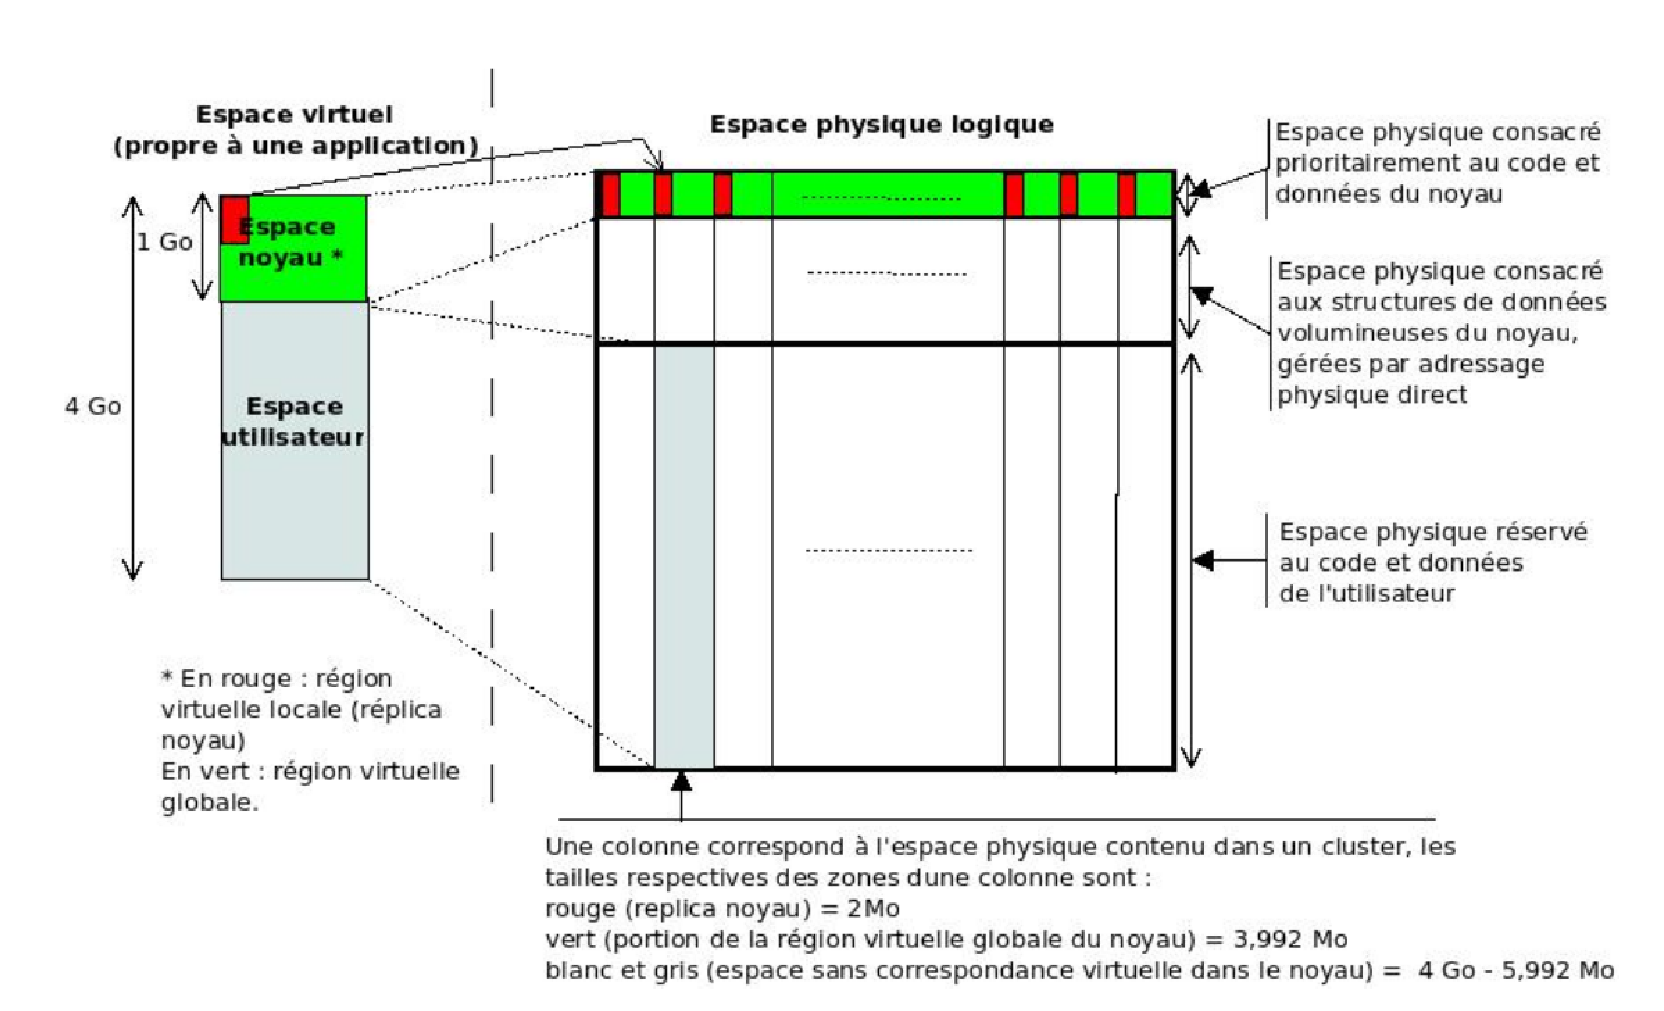
\includegraphics[scale=0.8]{include/img/almos-guerret}
        \caption{Répartition de l'espace virtuel du noyau tel que proposé par
          Franćois \citet{guerret2014exploitation}.}
        \label{fig:almos-guerret}
      \end{figure}

      \begin{paragraph}{Gestion en adressage physiques de structures de données:}
        Avec 4Mo d'espace virtuel pour le noyau par clusters, certaines
        structures de données ne pouvent plus être contenues dans un si petit
        espace, comme par exemple la table des pages. Celle-ci, une fois
        pleine\footnote{Ce cas n'arrive jamais, mais il est néanmoins
          théoriquement possible}, peut atteindre une taille maximale de 8Mo. De
        plus, chaque processus dispose de sa propre table des pages. Il est
        techniquement impossible de stocker 8Mo dans cet espace virtuel,
        François a donc choisi de sortir cette structure de l'espace virtuel.

        La seconde structure de données qui pose problème est la table des
        descripteurs de pages physiques. Les noyaux actuels ont fait le choix de
        décrire toutes les pages physiques qu'offre la mémoire. Ainsi, pour
        décrire le tera-octet de mémoire offert par TSAR, il est nécessaire
        d'utiliser 14Go de mémoire, soit 56Mo par cluster. Une fois de plus, il
        est impossible de stocker cette structure dans l'espace virtuel
        noyau. Celle-ci en a donc été sortie et est gérée en adressage physique.
      \end{paragraph}

      \begin{paragraph}{Résultats:}
        Ce travail n'a malheureusement pas donné lieu à une solution
        fonctionnelle. La gestion par des adresses physiques des ce deux
        structures s'est avérée être très compliquée et nécessitait de recoder
        une partie conséquente du noyau. Le principal inconvénient de ce choix
        est le parcours de listes: il est nécessaire de vérifier que chaque
        élément n'est pas une structure gérée physiquement avant de pouvoir
        l'accéder. Cela allourdi considérablement l'opération, cette solution
        fût donc abandonnée. Néanmoins, elle a ouvert la voie à la version
        suivante d'ALMOS.
      \end{paragraph}

      
  \section{Passage au mode multi-noyau}
  \label{sec:multi-noyau}

    La version actuelle d'ALMOS proposée par Mohamed Karaoui et Franck Wajsbürt
    supprime totalement l'espace virtuel du noyau. Ce dernier fonctionne
    entièrement en adressage physique et passe en mode multi-noyau, avec une
    instance de noyau dans chaque cluster. Ces changements permettent de gérer
    toute la mémoire physique de la plateforme TSAR, puisque \benumline \item
    chaque cluster dispose de 4Go de mémoire physique \item on a un noyau par
    cluster \item le noyau peut gérer 4Go de mémoire\eenumline. Ce changement
    permet également de laisser 4Go de mémoire virtuelle\footnote{Modulo une
      page de petite taille (4Ko) pour faire le passage entre le mode
      utilisateur et le mode noyau} à l'utilisateur puisque le noyau ne
    l'utilise plus.\\

    En revanche, cette solution possède un inconvénient majeur. En choisissant
    de clusteriser le noyau, on rend impossible la communication directe à la
    mémoire des clusters voisins. En effet, avec un noyau par cluster, les
    espaces d'adressage deviennent propres à ces derniers, et la vision d'un
    espace d'adressage unique entre les clusters n'existe plus. On ne peut donc
    plus accéder aux éléments des autres clusters de manière directe et
    transparente. La seule méthode est d'utiliser le passage de messages entre
    les instances du noyau.\\

    Une seconde conséquence de ce choix est d'avoir rendu non fonctionnelle la
    migration de processus et de threads entre les clusters (la migration entre
    c\oe urs d'un même cluster l'est toujours). Dans la version initiale
    d'ALMOS, cette migration se faisait\benumline \item en stoppant le processus
    sur le c\oe ur concerné \item en l'ajoutant dans la liste des processus du
    c\oe ur distant \item en relancant son exécution sur ce nouveau c\oe
    ur\eenumline. L'ajout du processus dans cette liste est possible uniquement
    parce que le noyau est en mémoire virtuelle. Il peut ainsi accéder au
    \textit{core-manager} du cluster destinataire, sans se rendre compte que
    celui-ci est distant, et lui ajouter la \texttt{struct task} du processus à
    migrer. Les pages physiques du processus seront ensuite migrées via la
    stratégie \textit{Auto-Next-Touch\footnote{Non détaillée dans ce
        rapport. Voir~\citep{almaless2014universite}.}}.

    En choisissant de passer ALMOS en mode multi-noyau, les clusters sont tous
    gérés par un noyau différent, et ont par conséquent des espaces d'adressage
    différents. Les mécanismes de migration ne sont donc plus applicables dans
    cette situation puisque qu'un noyau ne peut accéder qu'au 4Go de son
    cluster.


    \subsection{Traduction d'adresses}

      Si les processus utilisateurs utilisent toujours la mémoire virtuelle, ce
      n'est plus le cas du noyau. Nous allons voir comment celui-ci peut
      construire et manipuler des adresses sur 40 bits alors qu'il n'en dispoe
      que de 32 dans ses registres.

      \begin{paragraph}{Les processus utilisateurs:}
        Comme pour les autres noyaux, la traduction des adresses virtuelles en
        adresses physiques sont faites par la MMU. Tout ce processus est
        entièrement géré par le matériel. Le processeur n'a pas conscience qu'il
        manipule des adresses virtuelles. Dans l'architecutre TSAR, la tables
        des pages est composées de deux niveaux d'indirections
        (figure~\ref{fig:page-table}).
        
        \begin{figure}[ht]
          \centering
          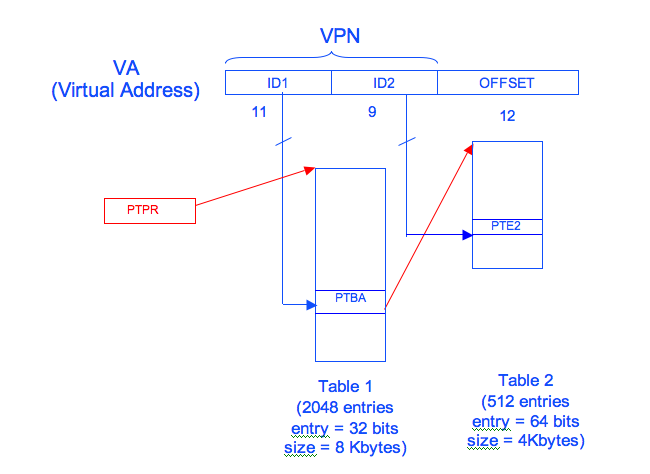
\includegraphics[scale=0.35]{include/img/pages_table_levels.png}
          \caption{La table des pages et sa
            hiérarchie~\citep{tsar2008web}.}
          \label{fig:page-table}
        \end{figure}
        \FloatBarrier
      \end{paragraph}
      
      \begin{paragraph}{Le noyau:}
        Lors du passage en mode noyau, la MMU est désactivée. A partir de cet
        instant, toutes les adresses manipulées par le processeur seront des
        adresses physiques. Or, celles-ci sont sur 32 bits. Pour contourner
        cette limite, ALMOS exploite deux caractéristiques \benumline \item les
        processeurs récents disposent des registres d'extension d'adresses \item
        l'architecture clusterisée de TSAR numérote ces derniers par un système
        de coordonnées $cid = (x, y) | 0 \leq x,y \leq 255$ \eenumline. On va
        donc concaténer $x$ et $y$ à l'adresse physique sur 32 bits, pour
        obtenir une adresse physique sur 40 bits.
      \end{paragraph}

      
  \section{Objectifs}

    La problématique soulevée en~\ref{sec:multi-noyau} est celle à laquelle nous
    allons répondre dans le cadre de ce stage. Plus précisément, il s'agit de
    définir et de mettre en place les mécanismes suivants:
    
    \begin{itemize}
      \item assurer la création et la migration de processus mono-threads entre
        clusters
      \item ajouter le support du multi-threading
      \item ré-implémenter le composant d'ALMOS appelé DQDT (Distributed
        Quaternary Decision Tree), assurant la vision globale de l'occupation
        des ressources matérielles de la plateforme, et par conséquent
        reponsable du placement des ressources sur celle-ci.
    \end{itemize}
